%
%
%%%%%%%%%%%%%%%%%%%%%%%%%%%%%%%%%%%%%%%%%%%%%%%%%%%%%%%%%%%%%%%%%%%%%%%%%%%%%
% We first setup margins for EuMW papers.
% This is done before the \documentclass is invoked.
%
\newcommand{\CLASSINPUTtoptextmargin}{19mm}%
\newcommand{\CLASSINPUTbottomtextmargin}{43mm}%
\newcommand{\CLASSINPUTinnersidemargin}{12.9mm}%
\newcommand{\CLASSINPUToutersidemargin}{12.9mm}%
%
%%%%%%%%%%%%%%%%%%%%%%%%%%%%%%%%%%%%%%%%%%%%%%%%%%%%%%%%%%%%%%%%%%%%%%%%%%%%%
%
% requires IEEEtran V1.8+, as hosted on CTAN at the following URL:
%	http://www.ctan.org/tex-archive/macros/latex/contrib/IEEEtran/
%
\documentclass[conference,10pt,a4paper]{IEEEtran}%CP this assumes IEEEtran V1.8+
%
%%%%%%%%%%%%%%%%%%%%%%%%%%%%%%%%%%%%%%%%%%%%%%%%%%%%%%%%%%%%%%%%%%%%%%%%%%%%%
% Now we import required packages
%
\usepackage{amsmath}% for double integral symbol in this template
\usepackage{times}% use times font for the paper instead of default LaTeX fonts
\usepackage{graphicx}% for figures
\usepackage{multirow}% to allow multiple-row elements in tabular environment
\usepackage[none]{hyphenat}% turn off hyphenation to make text extraction and indexing easier
\usepackage{float}% better control of floating figures and tables
\usepackage{subfig}% for labelling subfigures within figures
\usepackage{iftex}% for detecting whether XeLaTeX or pdfLaTeX is being used, for the purpose of choosing the right fonts below.
\usepackage{xurl}% use this package to manage long urls in the references section
\usepackage{svg}% for including SVG images
\usepackage{booktabs}       % for \toprule, \midrule, \bottomrule, \addlinespace                                       
\usepackage[table]{xcolor}  % for \cellcolor 
%
%%%%%%%%%%%%%%%%%%%%%%%%%%%%%%%%%%%%%%%%%%%%%%%%%%%%%%%%%%%%%%%%%%%%%%%%%%%%%
% users of pdfLaTeX must uncomment the following lines:
\ifPDFTeX%
\usepackage{t1enc}% allows access to various special characters
\usepackage{times}% change font to Nimbus Roman (based on Times Roman)
\fi%
%%%%%%%%%%%%%%%%%%%%%%%%%%%%%%%%%%%%%%%%%%%%%%%%%%%%%%%%%%%%%%%%%%%%%%%%%%%%%
% users of XeLaTeX or LuaTeX must uncomment the following two lines:
\ifXeTeX%
\usepackage{fontspec}% needed to change main font
\setmainfont{TeX Gyre Termes}% change font to TeX Gyre Roman (based on Times Roman)
\fi%
%%%%%%%%%%%%%%%%%%%%%%%%%%%%%%%%%%%%%%%%%%%%%%%%%%%%%%%%%%%%%%%%%%%%%%%%%%%%%
% users of pdfLaTeX must uncomment the following lines:
\ifLuaTeX%
\usepackage{fontspec}% needed to change main font
\setmainfont{TeX Gyre Termes}% change font to TeX Gyre Roman (based on Times Roman)
\fi%
%%%%%%%%%%%%%%%%%%%%%%%%%%%%%%%%%%%%%%%%%%%%%%%%%%%%%%%%%%%%%%%%%%%%%%%%%%%%%
%
%%%%%%%%%%%%%%%%%%%%%%%%%%%%%%%%%%%%%%%%%%%%%%%%%%%%%%%%%%%%%%%%%%%%%%%%%%%%%
% Next we modify the standard IEEEtran.cls format to produce EuMW format by 
% redefining some macros.
\input{EuMW_modify_IEEEtran_18b_CTAN_V6}
%%%%%%%%%%%%%%%%%%%%%%%%%%%%%%%%%%%%%%%%%%%%%%%%%%%%%%%%%%%%%%%%%%%%%%%%%%%%%
%
%%%%%%%%%%%%%%%%%%%%%%%%%%%%%%%%%%%%%%%%%%%%%%%%%%%%%%%%%%%%%%%%%%%%%%%%%%%%%
\begin{document}
%%%%%%%%%%%%%%%%%%%%%%%%%%%%%%%%%%%%%%%%%%%%%%%%%%%%%%%%%%%%%%%%%%%%%%%%%%%%%
% We use \raggedbottom to avoid latex adding vertical space around headings.
% This gives a better idea to the author about how much white space remains
% as the page limit is approached.
\raggedbottom
%
%%%%%%%%%%%%%%%%%%%%%%%%%%%%%%%%%%%%%%%%%%%%%%%%%%%%%%%%%%%%%%%%%%%%%%%%%%%%%
% PAPER TITLE AND AUTHOR BLOCK
%
% The paper title can use linebreaks \\ within to get better formatting if desired.
%
\title{Design and Implementation of Tracking Filters for a Passive Radar System}
%
% Next we define the author names and affiliations.
\author{%
\IEEEauthorblockN{%
Itumeleng Malemela\EuMWauthorrefmark{\#1\textasciicircum 2}, 
Stephen Paine\EuMWauthorrefmark{\#1}, 
Francois Schonken\EuMWauthorrefmark{\#1}
}% \IEEEauthorblockN Names
\IEEEauthorblockA{%
\EuMWauthorrefmark{\#1}Department of Electrical Engineering, University of Cape Town, South Africa\\
\EuMWauthorrefmark{\textasciicircum 2}Council for Scientific and Industrial Research (CSIR), South Africa\\
\{\EuMWauthorrefmark{1}mlmitu002, \EuMWauthorrefmark{1}stephen.paine, \EuMWauthorrefmark{1}francois.schonken\}@uct.ac.za, 
\EuMWauthorrefmark{2}imalemela@csir.co.za
}% \IEEEauthorblockA
}% \author
% Next we make the title/author block using the information defined above.
\maketitle
%
%%%%%%%%%%%%%%%%%%%%%%%%%%%%%%%%%%%%%%%%%%%%%%%%%%%%%%%%%%%%%%%%%%%%%%%%%%%%%
% ABSTRACT paragraph.
%
% As a general rule, do not put math, special symbols or citations
% in the abstract paragraph.
%
\begin{abstract}
Passive Radar exploits existing transmitter infrastructure to detect targets through their skin returns. FM Passive Radar offers high Doppler resolution due to the available longer integration times but faces challenges, including clutter, direct and multipath interference, and low range resolution due to the low bandwidth. While tracking filters have been widely studied, their application to commercial aircraft tracking using FM signals in the bistatic range Doppler domain remains limited. This paper presents the design and evaluation of four tracking filters, namely the Kalman, Unscented Kalman, Particle, and Recursive Gauss-Newton filters, incorporating an adaptive covariance scaling mechanism to handle outliers and zero-Doppler cancellation artefacts. Filters are assessed through a log likelihood statistical benchmark and computational load using the Flexible Extensible Radar Simulator in a multi-target scenario context. The Recursive Gauss-Newton Filter achieves the best log likelihood performance while meeting real-time constraints.
\end{abstract}
\begin{IEEEkeywords}
adaptive filters, FM Passive Radar, Kalman filters, Recursive Gauss-Newton filter, Particle filter, log likelihood, Radar tracking filters
\end{IEEEkeywords}
%
%%%%%%%%%%%%%%%%%%%%%%%%%%%%%%%%%%%%%%%%%%%%%%%%%%%%%%%%%%%%%%%%%%%%%%%%%%%%%
% THE REST OF THE PAPER follows.
%

\section{Introduction}

Ever since the emergence of Radio Detection and Ranging (Radar) technology, there has been a tremendous evolution in Radar systems. Modern Radar systems are now capable of not only detecting and determining range but also tracking, identifying, and classifying targets in cluttered environments \cite{Richards2010}. Passive Radar (PR) systems detect and track objects by passively receiving and analysing signals from external sources, known as illuminators of opportunity, including FM radio, DVB-T, and cellular broadcasts \cite{Howland2005a}. This characteristic allows PR systems to operate without emitting any signals, making them advantageous for covert operations and cost-effective applications.

This research focuses on tracking targets using PR systems leveraging Frequency Modulation (FM) radio signals as illuminators of opportunity. FM signals offer widespread availability, robustness to weather-induced degradation, and no spectrum licensing requirements, making FM PR attractive for cost-effective air traffic control at small airports in developing countries.

Specifically, this work designs and evaluates four tracking filters for commercial aircraft tracking in the bistatic range and Doppler domain using FM PR, incorporating an adaptive covariance scaling mechanism and a log likelihood (LL) based performance assessment across simulated flight scenarios.                                                                                                                                       
%%%%%%%%%%%%%%%%%%%%%%%%%%%%%%%%%%%%%%%%%%%%%%%%%%%%%%%%%%%%%%%%%%%%%%%%%%%%%

\section{System Overview}

The simulation framework comprises four key stages: the Radar environment, modelled using FERS; the Radar processing chain; the tracking filters; and the Multi-Target Tracking (MTT) system, as depicted in Fig.~\ref{fig:radarOverview}.                    
                  
\begin{figure}[H]                                          
    \centering
    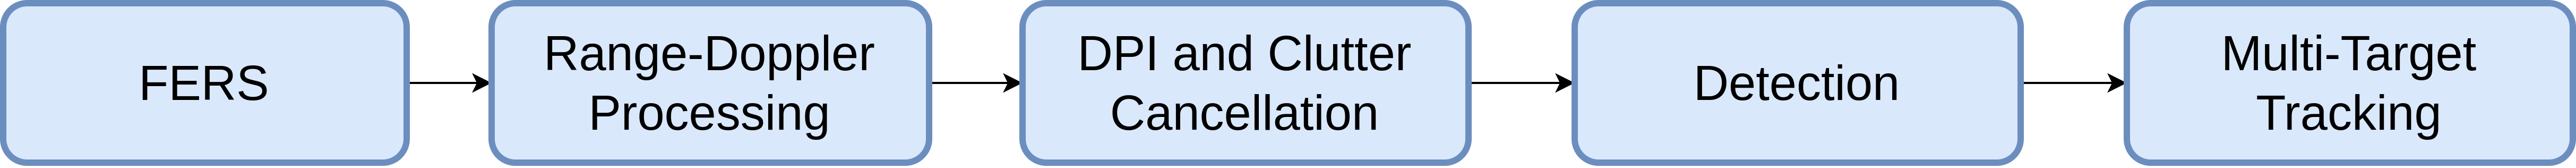
\includegraphics[width=1\linewidth]{figures/radarOverview.drawio.png}        
    \caption{Radar System Overview.}                                             
    \label{fig:radarOverview}
\end{figure}                                                                                                                                            
\subsection{Flexible Extensible Radar Simulator}

FERS is used to simulate the behaviour of the Radar system. FERS was developed from a Ph.D. thesis presented in \cite{fersMarc}, which was based on creating a simulator that supports various Radar system configurations. A bistatic Radar configuration is modelled with one transmitter, two receivers (reference and surveillance), and targets, as illustrated in Fig.~\ref{fig:360_3D}. The transmitter is simulated as an omni-directional FM illuminator with a centre frequency of 94~MHz using an isotropic antenna, while the receivers employ directional antennas. The transmitter-receiver
baseline is 12.5~km.                                                                           
\subsection{Radar Processing Chain}                                                                        
From the FERS output files, the reference and surveillance signals are reconstructed into complex baseband form. The Amplitude Range Doppler (ARD) map is computed in discrete time as:
\begin{equation}                                                         
  \left| \Psi(\tau, v) \right| = \left| \sum_{n=0}^{N-1} s_E(n) s_R^*(n-\tau) e^{j 2\pi v n/N} \right|                                                 
\end{equation}                                                                                                                                           
where $\Psi(\tau, v)$ is the ARD map, $s_E(n)$ represents the echo signal, and $s_R^*(n-\tau)$ is the complex conjugate of the reference signal. Range-Doppler processing utilizes 200 kilosamples per second.                                                                                            

To improve detection performance, Direct Path Interference (DPI) and clutter are suppressed from the surveillance channel prior to range-Doppler processing. For this purpose, the Extensive Cancellation Algorithm (ECA), based on the least mean squares estimator, is applied due to its fast convergence and demonstrated effectiveness in clutter suppression \cite{coloneECA}. The target detection stage evaluates each cell in the range-Doppler map against an adaptive threshold using a Cell Averaging Constant False Alarm Rate (CA-CFAR) detector, which allows tuning of the detection probability through the probability of false alarm $P_{fa}$. Because the target spans multiple range bins due to the limited bandwidth of the FM waveform, averaging is applied only in the Doppler domain, where higher resolution is available.       
              
The CFAR output produces multiple detections across adjacent Doppler and range cells. To generate measurements suitable for tracking, these detections are grouped into clusters using mean-shift clustering, which does not require prior knowledge of the number of targets and directly provides cluster centroids \cite{cheng1995mean}. The bandwidths used are 5 Hz and 10 km for the Doppler and range dimensions, respectively.
%%%%%%%%%%%%%%%%%%%%%%%%%%%%%%%%%%%%%%%%%%%%%%%%%%%%%%%%%%%%%%%%%%%%%%%%%%%%%

\begin{figure*}[t]                                    
\centering                                            
\subfloat[]{%                                          
  \includesvg[width=0.38\linewidth,inkscapelatex=false]{figures/3D_360.svg}%                              
  \label{fig:360_3D}%                                      
}%                                                       
~
\subfloat[]{%
  \includesvg[width=0.38\linewidth,inkscapelatex=false]{figures/360_filter_output.svg}%
  \label{fig:360FilterOutputs}%
}%
\\[2.6mm]
\caption{360-degree manoeuvre scenario: (a) bistatic Radar geometry in the FERS simulation showing Tx, SurvRx, and RefRx positions with the target trajectory in Cartesian coordinates; (b) tracking filter predictions, measurements, and ground truth in the bistatic range and Doppler domain.}
\label{fig:360_scenario}
\end{figure*}

\section{Tracking Filters and Adaptive Filtering}                                         
\subsection{Doppler Range Target Tracking}
The centroids obtained from clustering provide estimates of the target's position in the bistatic range Doppler domain. To track the target state, a Nearly Constant Velocity (NCV) model is adopted, which is suitable for non-manoeuvring targets such as commercial aircraft, where abrupt changes in range or Doppler are unlikely \cite{Li2003a}. The NCV state vector is defined as:                                                                   
\begin{equation}
  x(t) = [r_t, \dot{r_t}, f_t, \dot{f_t}]^T,                                    
\end{equation}                                                                                                                                           
where $r_t$ and $f_t$ denote bistatic range and Doppler, and $\dot{r_t}, \dot{f_t}$ their rates. The discrete time evolution is                          
\begin{equation}                                                               
  \mathbf{X}_k =
  \begin{bmatrix}                                                   
      1 & \tau & 0 & 0 \\
      0 & 1 & 0 & 0 \\                                              
      0 & 0 & 1 & \tau \\                                           
      0 & 0 & 0 & 1                                               
  \end{bmatrix} X_{k-1} + w_{k-1},                            
\end{equation}                                                
with sampling interval $\tau$ and zero mean Gaussian process noise $w_{k-1}$ whose covariance is:                                            
\begin{equation}                                               
  Q = S_w     
  \begin{bmatrix}                                              
      \tfrac{\tau^4}{4} & \tfrac{\tau^3}{2} & 0 & 0 \\
      \tfrac{\tau^3}{2} & \tau^2 & 0 & 0 \\                        
      0 & 0 & \tfrac{\tau^4}{4} & \tfrac{\tau^3}{2} \\             
      0 & 0 & \tfrac{\tau^3}{2} & \tau^2                          
  \end{bmatrix},                                               
\end{equation}                                                                                                                                           
where $S_w$ denotes the process noise spectral density \cite{Measurements2023b}. Small values of $S_w$ correspond to NCV dynamics, whereas larger values capture manoeuvring behaviour \cite{953264}.                                                                                                        
\subsection{Tracking Filters Overview}
The Kalman Filter (KF) provides the linear Gaussian baseline and is valued for its computational efficiency and robustness \cite{Julier1997a}. The Unscented Kalman Filter (UKF) uses the unscented transform to propagate sigma points through non-linear functions without requiring Jacobians \cite{Julier1997a}. The Particle Filter (PF) uses Monte Carlo methods to represent the posterior distribution, offering a robust alternative when both the system dynamics and noise are highly non-linear and non-Gaussian \cite{Arulampalam2007, NJGordon}. The Recursive Gauss-Newton Filter (RGNF) aims to improve numerical performance and adaptivity to unknown dynamics, and has demonstrated effectiveness in both non-linear tracking scenarios and linear cases such as Doppler-only and bistatic Radar tracking \cite{Inggs1, De2015, roaldje}.

\subsection{Log Likelihood}                                    
The LL is used as a statistical benchmark to evaluate each filter's performance. Unlike Root Mean Square Error (RMSE), which evaluates only the filter outputs, the LL incorporates the error covariance matrix $\mathbf{P}$, providing a measure of both estimation accuracy and filter uncertainty \cite{labbe2014kalman, Grewal2006}. The LL at time step $k$ is defined as:
\begin{equation}                                               
  \ell_k = -\frac{1}{2}\left[\ln|S_k| + e_k^T S_k^{-1} e_k + n\ln(2\pi)\right],          
\end{equation}                                                                                                                                         
where $S_k = H_k P_k^- H_k^T + R_k$ is the innovation covariance, $e_k = z_k - H_k \hat{X}_k^-$ is the innovation, and $n$ is the dimension of the       
measurement vector.                                                                                                                                     
\subsection{Adaptive Filtering}                               
Accurate state estimation depends on the appropriate selection of the measurement noise covariance $\mathbf{R}$ and process noise covariance $\mathbf{Q}$. Fixed values of these matrices may degrade tracking performance under deviations from the assumed motion model or in the presence of outliers, which is particularly relevant in the tracking of commercial aircraft to achieve stable and smooth trajectory estimates. Adaptive filtering addresses this limitation by adjusting $\mathbf{R}$ and $\mathbf{Q}$ during operation \cite{Mehra1972}. Among several approaches, covariance matching is adopted in this work.

The covariance scaling method updates for $\mathbf{R}$ and $\mathbf{Q}$ using the innovation and residual, defined as:                                        
\begin{equation}
  d_k = z_k - h_k(\hat{X}^-_k), \quad \varepsilon_k = z_k - h_k(\hat{X}^+_k),
\end{equation}                                                                                                                                          
where $z_k$ is the measurement, and $\hat{X}^-_k, \hat{X}^+_k$ are the predicted and estimated states respectively. For adaptive estimation of $\mathbf{R}$, the innovation covariance is:                                                                                                               
\begin{equation}                                               
  S_k = H_k P^-_k H_k^T + R_k,                                 
\end{equation}                                              
leading to the update:
\begin{equation}                                               
  R_k = \alpha R_{k-1} + (1-\alpha)(\varepsilon_k \varepsilon_k^T + H_k P^-_k H_k^T),
\end{equation}                                                 
where $0 \leq \alpha \leq 1$ is a forgetting factor \cite{Akhlaghi2018}. This formulation enables the filter to adapt measurement noise statistics online and maintain robustness against outliers or unexpected dynamics.                                                                 
                 
\subsection{Multi Target Tracking}  
In practical scenarios, multiple detections may arise within a single processing interval, requiring association with existing tracks and effective track management. The implemented MTT framework consists of gating, Global Nearest Neighbour (GNN) association, and an M out of N track management strategy. Gating rejects unlikely detection-to-track associations using an ellipsoidal validation region based on the Mahalanobis distance                         
\cite{Jerrelind2020,Richards2010}:
\begin{equation}                                 
  Z_k S_k^{-1} Z_k^T \leq G,
\end{equation}                                                                                                                      
where $Z_k$ is the measurement residual, $S_k = H_k P_k H_k^T + R_k$ the innovation covariance, and $G$ the gating threshold. Observations within the gate are assigned using the GNN method, which minimizes the distance measure \cite{Konstantinova2003}:
\begin{equation}
  d^2_{G_{ij}} = d^2_{ij} + \ln|S_i|.                          
\end{equation}                                                 
Unassigned detections are used to initiate new tracks. Track confirmation is based on the M out of N rule, in which a track is promoted from tentative to confirmed if a detection is observed in at least $M$ of the last $N$ scans.  
%%%%%%%%%%%%%%%%%%%%%%%%%%%%%%%%%%%%%%%%%%%%%%%%%%%%%%%%%%%%%%%%%%%%%%%%%%%%%

\section{Simulations and Results}
The tracking filters are evaluated across three FERS flight scenarios representing common commercial aircraft manoeuvres in
the bistatic range and Doppler domain: a straight and level flight (60~s), a landing manoeuvre with descent and turn (120~s), and a 360-degree orbit (120~s). The covariance scaling mechanism is applied to all filters to mitigate outliers from zero-Doppler cancellation artefacts and range smearing inherent to FM waveforms.

\subsection{360-Degree Manoeuvre}
The 360-degree manoeuvre, illustrated in Fig.~\ref{fig:360_scenario}(a), represents a common holding pattern for commercial aircraft at constant altitude. The closed-loop bistatic range and Doppler trajectory in Fig.~\ref{fig:360_scenario}(b) presents a challenging scenario due to continuous rate changes in both domains. All four   
filters successfully track the target through the full orbit, with the RGNF and KF maintaining the most stable range LL. Range predictions show a slight offset from ground truth, as measurement covariance is configured with lower range sensitivity to mitigate FM bandwidth-induced fluctuations.

\subsection{Log-Likelihood Evaluation}                                   
The LL is used as the primary performance metric to evaluate the tracking filters across all three flight scenarios. Higher (less negative) values indicate better statistical consistency between the filter estimates and the ground truth. As the filters converge, the error covariance matrix $\mathbf{P}$ decreases and the LL approaches zero, reflecting increasing confidence in the state estimates.

\begin{figure}[t]                                                 
  \centering
  \includesvg[width=0.7\linewidth,inkscapelatex=false]{figures/360_doppler_ll.svg}
  \caption{Doppler LL for the 360-degree manoeuvre scenario.}
  \label{fig:dopplerLogLike360}
\end{figure}

Fig.~\ref{fig:dopplerLogLike360} shows the Doppler LL for the 360-degree scenario. The RGNF maintains the most stable
values throughout, while the UKF exhibits significant dips during the turns as its sigma-point spread amplifies the effect 
of corrupted Doppler measurements. The KF and PF show consistent behaviour, though the PF produces a lower overall LL
due to the variance inherent in particle-based estimation. Table~\ref{tab:ll_ranking} presents the ranked LL performance   
across all three flight scenarios.                                          
\begin{table}[t]                                                   
\centering
\caption{Ranked LL performance across flight scenarios (1 = best, 4 = worst).}
\label{tab:ll_ranking}
\setlength{\tabcolsep}{3pt}
\begin{tabular}{@{}llcccc@{}}
\toprule
\textbf{Scenario} & \textbf{Domain} & \textbf{KF} & \textbf{UKF} & \textbf{PF} & \textbf{RGNF} \\
\midrule
Landing & Range   & 2 & 3 & \cellcolor{red!20}4 & \cellcolor{green!20}\textbf{1} \\
      & Doppler & 3 & \cellcolor{green!20}\textbf{1} & \cellcolor{red!20}4 & 2 \\
\addlinespace
360\textdegree & Range   & 3 & \cellcolor{green!20}\textbf{1} & \cellcolor{red!20}4 & 2 \\
             & Doppler & 3 & 2 & \cellcolor{red!20}4 & \cellcolor{green!20}\textbf{1} \\
\addlinespace
Take-off & Range   & 2 & 3 & \cellcolor{red!20}4 & \cellcolor{green!20}\textbf{1} \\
       & Doppler & 2 & \cellcolor{green!20}\textbf{1} & \cellcolor{red!20}4 & 3 \\
\bottomrule
\end{tabular}
\end{table}
The RGNF consistently achieves the highest LL across scenarios, with its iterative Gauss-Newton update enabling rapid convergence. The KF offers comparable stability with minimal computational overhead. The UKF demonstrates strong Doppler LL but is sensitive to outlier measurements during manoeuvres. The PF ranks last, as particle-based estimation variance limits its LL performance despite using 10\,000 particles. 

\subsection{Computational Load}
Table~\ref{tab:comp_load} presents the relative computational load of each filter, where the relative load is defined as the ratio of the average runtime of each filter to the average runtime of the KF. Processing times were averaged over 1\,000 Monte Carlo simulations of a 60\,s single-target scenario.                                                     
\begin{table}[H]                                                  
  \centering                                                      
  \caption{Relative computational load of each tracking filter.}       
  \label{tab:comp_load}
  \begin{tabular}{@{}lcc@{}}
  \toprule
  \textbf{Filter} & \textbf{Update} & \textbf{Prediction} \\
  \midrule
  KF   & 1.00 & 1.00 \\
  UKF  & 0.96 & 1.39 \\
  PF   & 6.53 & 3.56 \\
  RGNF & 1.12 & 1.08 \\
  \bottomrule
  \end{tabular}
\end{table}

All filters satisfy real-time constraints for single-target tracking, with per-scan processing times in the microsecond range, well below typical coherent processing intervals of 0.5--1\,s \cite{Howland2005a}. Fig.~\ref{fig:mtt_output} illustrates the MTT output for a three-target scenario using the KF with GNN association and 3-out-of-4 M-out-of-N track management.                                                                      
\begin{figure}[H]
    \centering
    \includesvg[width=0.7\linewidth,inkscapelatex=false]{figures/mtt_3_tracking_corrections_v1.svg}
    \caption{MTT output using a KF with GNN association and 3-out-of-4 M-out-of-N track management for a three-target
scenario.}
    \label{fig:mtt_output}
\end{figure}

In an MTT framework, each confirmed track requires an independent filter instance, with total cost scaling linearly with the number of targets. For the PF, with an update stage 6.53$\times$ that of the KF, this scaling limits its suitability for real-time MTT. The overhead of gating, GNN association, and track management further constrains the computational budget \cite{Konstantinova2003}. The KF and RGNF offer the most favourable balance between accuracy and computational feasibility for MTT deployment.
%%%%%%%%%%%%%%%%%%%%%%%%%%%%%%%%%%%%%%%%%%%%%%%%%%%%%%%%%%%%%%%%%%%%%%%%%%%%%

\section{Conclusion}

This paper presented four tracking filters, namely the KF, UKF, PF, and RGNF, for FM PR commercial aircraft tracking in the bistatic range-Doppler domain, incorporating adaptive covariance scaling to mitigate outliers from zero-Doppler cancellation and FM bandwidth limitations. The RGNF achieved the best LL performance with computational loads near the KF baseline, while the KF offered comparable stability at lowest cost. The UKF demonstrated strong Doppler tracking but sensitivity to outliers during manoeuvres, and the PF ranked last in both LL and computational efficiency. Future work includes validating with real-world PR system data, exploring deep learning methods for complex target dynamics, and optimization techniques for tracking filter tuning.
%%%%%%%%%%%%%%%%%%%%%%%%%%%%%%%%%%%%%%%%%%%%%%%%%%%%%%%%%%%%%%%%%%%%%%%%%%%%%

%\section*{Acknowledgment}
%The authors would like to thank Dr.\ Willem Schonken and Dr.\ Stephen Paine of the University of Cape Town for their supervision and guidance.

%%%%%%%%%%%%%%%%%%%%%%%%%%%%%%%%%%%%%%%%%%%%%%%%%%%%%%%%%%%%%%%%%%%%%%%%%%%%%

\bibliographystyle{IEEEtran}

\bibliography{IEEEabrv,IEEEexample}

\end{document}


